\section{Forecasting}
\label{sec:forecast}

\Opensolutionfile{ans}

\textit{Recommended reading:} FP Section 13.3. FP describes various methods and concepts related to demand forecasts, e.g. regression, moving-averages, exponential smoothing, trends and seasonal patterns, measures of forecast accuracy. We expect you to be familiar with these basic methods. 

Any successful inventory management practice starts with projecting the demand that will realize in the future. This section is devoted to understanding demand processes and forecasting future demands. 

\begin{exercise}
Why inventories are replenished ahead of demand?


  \begin{solution}
    There is a variety of reasons. For instance, often there is an order lead time, i.e. the lag between the time that an order is placed and the time inventory is actually replenished. Another reason is that it could be preferable to place larger orders due to economies of scale, e.g. quantity discounts or fixed ordering costs. 
    
	Let us consider an inventory system where replenishments are done on a daily basis. That is, you place an order at the end of every day, and receive it the next day in the morning. It appears that there is no lead time here. But anyway you are exposed to demand uncertainty over the day. That is, you must have enough in the morning to cover the demand over the day -- which has not yet been realized. 
  \end{solution}
\end{exercise}


\subsection{The Role of Demand Forecasts}

\begin{exercise}
Why do we need to forecast demands?



  \begin{solution}
    We often need to replenish inventories ahead of demand, i.e. before observing the demand. As such, projection of future demands, or in other words, forecasting, is the foundation upon which replenishment plans are made. 
    
    Of course, in some cases, you might have the complete demand information before it is realized. For instance, your customers may let you know in advance, say a week before, they actually demand an item. In such cases, you can safely assume that you know the demand over the next week with certainty. Thus there will be no need for forecasting -- at least not for the upcoming week. 
  \end{solution}
\end{exercise}


\begin{exercise}
What should we expect from demand forecasts?



  \begin{solution}
	For most products, demand is inherently uncertain. As such, exact demand values cannot be forecasted. The aim of forecasting therefore is to capture the structural properties of demand, such as its average, rather than the demand itself.  
	

  \end{solution}
\end{exercise}

\begin{exercise}
Which factors come into play in forecasting, i.e. what is the input?



  \begin{solution}
    The input of forecasting is comprised of all type of information regarding historical demand as well as the future demand. These involve, among others, objective factors such as past demand data, trend and seasonality, prices, promotions, dependencies among different products, as well as subjective factors such as sales force surveys and expert opinions.     
  \end{solution}
\end{exercise}


\begin{exercise}
What is the output of a forecast?



  \begin{solution}
    The output of a forecast is a set of data points for future demands as well as a measure that explains to which extent actual demands will deviate from their forecasts.
  \end{solution}
\end{exercise}


\begin{exercise}
How are forecasts used inventory management?



  \begin{solution}
	Inventory management is done through inventory control policies. The output of forecasts are used in designing inventory control policies and determining the parameters of these policies.
  \end{solution}
\end{exercise}


\begin{exercise}
How much effort should be put into forecasting?



  \begin{solution}

	Because obtaining a highly accurate forecast is costly and time consuming, one should consider the trade off between its benefits and costs. The benefit of a forecast lies in how sensitive inventory costs are to forecast accuracy. 
	
	In inventory systems with a large number of SKU's it is simply not possible to put a lot of effort into forecasting. But for very expensive items which are sold rather infrequently (say a diamond ring or an aircraft spare part) the value of having a better forecast can be very high. This is mainly due to the cost of the mismatch between supply and demand, i.e. stock-out costs as well as holding costs are very high. 
	
	As a rule of thumb, one should avoid overly naive forecasting approaches as well as excessively complicated ones. 
  \end{solution}
\end{exercise}


\begin{exercise}\nvf{Move this to the eoq section}
Consider the EOQ problem (for the sake of simplicity neglect the unit production cost). Now assume that the demand $D$ that is used in computing the order quantity is off by a factor of $\Delta$. That is, actual demand happens to be $D(1+\Delta)$ rather than $D$. 
\begin{enumerate}
\item Derive an expression to illustrate the cost of using the wrong demand value as compared to the optimal cost. 
\item Plot the cost error for $-0.5\leq \Delta\leq 0.5$ and solution on the extent of the cost error.
\item Comment on the implications of this thought experiment with respect to the importance of forecast accuracy.
\end{enumerate}


  \begin{solution}
\begin{enumerate}
\item Because the order quantity is set assuming that demand is $D$, it will be $Q=\sqrt{2AD/h}$. If one were to know the real demand $D(1+\Delta)$, then the optimal order quantity would be $Q^*=\sqrt{2AD(1+\Delta)/h}$. 

Observe that  $Q^*=Q\sqrt{1+\Delta}$. That is, if demand is off by 20\% (i.e. $\Delta=0.2$) then the order quantity will be off by only 9.5\% (i.e. $Q^*/Q\approx 1.095$). When actual demand is $D(1+\Delta)$, the costs of using order quantities $Q^*$ and $Q$ will be 
\begin{align*}
C^* = AD\frac{1+\Delta}{Q^*} + h\frac{Q^*}{2} \quad \text{ and } \quad C = AD\frac{1+\Delta}{Q}+h\frac{Q}{2}
\end{align*}
respectively. Because, $Q^*$ is the optimal order quantity when demand is $D(1+\Delta)$, we have $C^*/2=AD(1+\Delta)/Q^*=hQ^*/2$. Hence $C^*=hQ^*$. The error $C/C^*$ can therefore be written as
\begin{align*}
\frac{C}{C^*} 
& = \frac{\frac{AD (1+\Delta)}{\sqrt{2AD/h}}+\frac{h\sqrt{2AD/h}}{2}}{h\sqrt{2AD/h}\sqrt{1+\Delta}} = \frac{1}{2}\left(\frac{1}{\sqrt{1+\Delta}} + \sqrt{1+\Delta}\right)
\end{align*}
\item See Figure~\ref{fig:costerror}. We observe that if demand is underestimated by 50\%, the cost error is 6\%; and if it is overestimated by 50\%, the cost error is 2\%. The cost penalty does not look that serious on the overall.

\begin{figure}
\centering
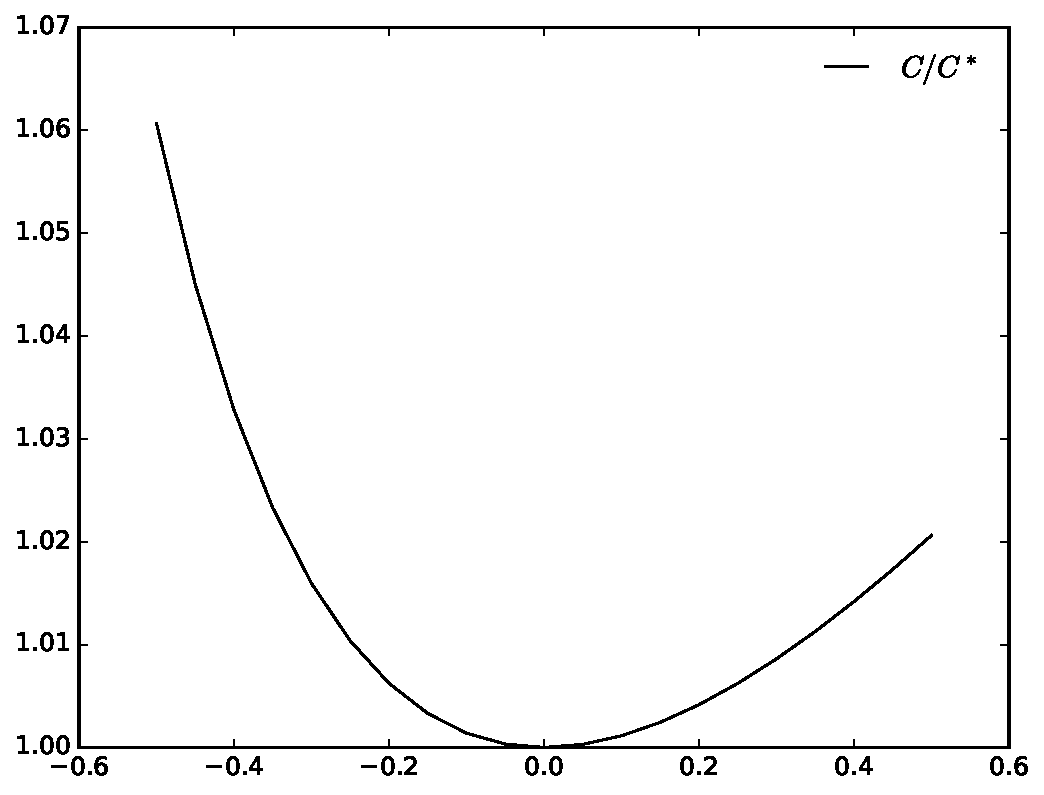
\includegraphics[width=.5\linewidth]{figures/Figure_1.pdf}
\caption{Cost error}
\label{fig:costerror}
\end{figure}

\item The EOQ cost is rather insensitive to the demand for which the order quantity is based upon. As such, a highly accurate forecast, although preferable, is not necessary. 
\end{enumerate}
    
  \end{solution}
\end{exercise}


\begin{exercise}
Discuss which underlying assumptions of the EOQ model make it insensitive to the demand uncertainty. 


  \begin{solution}
  The EOQ model assumes that all demand can be served in time. That is because the inventory will be replenished instantaneously whenever the inventory level drops down to zero. In that sense, not using the optimal order quantity effect the trade-off between the ordering and holding costs, but not the service quality. Often in stochastic inventory control systems there is a cost associated with providing a certain quality of service. This is not reflected on the EOQ model.
  \end{solution}
\end{exercise}

\subsection{Forecasting Methods}

\begin{exercise}
What type of methods are used in forecasting?


  \begin{solution}
    There are two types of forecasting methods: qualitative and quantitative methods. The former use subjective inputs such as expert opinions. These are more apt for long-term forecasts where past data are not sufficient to predict the future, e.g. where technological breakthroughs may play a significant role. The latter use objective inputs such as past data. These are more suitable for short-term forecasts where numerical measures of the past observations can explain the future with a sufficient degree of accuracy. 
   \end{solution}
\end{exercise}
   
\begin{exercise}
What type of forecasting methods are used in inventory management?



  \begin{solution}
	In most practical cases, the number of SKU's is too large to implement SKU-specific forecasting methods. As such, often automatized forecasting procedures that work solely with past quantitative data are employed for demand forecasting in inventory management. There are two types of quantitative forecasting models: causal models and time-series models.

   \end{solution}
\end{exercise}
   
\begin{exercise}
How do causal forecasting models work?



  \begin{solution}
    Causal models assume that demand is a function of some other parameters (e.g. price, market size, time, and weather). Here are some examples. The demand for diapers this year is a function of last years birth rates. The demand for FC Groningen jerseys is a function of the team and individual player performances. 

Once all the factors that explain demand are identified, one can easily predict demand given the values of these parameters. 

Let $X_1,X_2,\ldots,X_m$ be the values of the parameters explaining the demand. Then, assuming that each parameter effects the demand linearly and independently, the forecast would be 
\begin{equation*}
Y = b_0 + b_1 X_1 + \ldots + b_m X_m
\end{equation*}
where $b_0,b_1,\ldots,b_m$ are the constants defining the demand function. 

Here, the challenge is to find a function (i.e. the parameters values $b_0,b_1,\ldots,b_m$) that best forecasts the demand. This is often done by using past data via regression analysis -- a highly accessible tool as it is available in almost all spreadsheet programs. 

An important drawback of using a causal model is that the values of those parameters explaining demand should be readily available. Otherwise, one needs to to forecast them before forecasting demand. For instance, if the weather is a factor effecting the demand, then one needs the forecast the weather before forecasting the demand.    

  \end{solution}
\end{exercise}


\begin{exercise}
How do time-series forecasting models work?



  \begin{solution}
Time-series models assume that past demand data are almost sufficient to forecast future demands. As such, all causal factors are neglected with the rationale that such factors tend not to change in the short-term. 

If time is treated as a discrete entity (i.e. days, weeks, or months), then, assuming that period $t$ is the actual period, a time-series model takes all past demand observations $A(1),A(2),\ldots,A(t)$ and generates forecasts $f(t+1),f(t+2)\ldots$ for future demands. 

As compared to causal models, time-series models are more commonly used in inventory management because they are very simple, do not require much data, and (often) reliable. Also, they are easy to use and integrated in many spreadsheet applications.
  \end{solution}
\end{exercise}


\begin{exercise}
How exactly do time-series models forecast demand by solely using past demand data?



  \begin{solution}
There are two approaches towards time-series forecasting: moving-averages and exponential smoothing. The main idea behind both approaches is to put emphasis on the recent demand data when making a forecast, based on the belief that recent data better explains actual demand.

\textit{Moving-Averages:} 
Here, one simply averages recent demand data to forecast demand. Let us define 'recent' as the last $m$ periods. Then, the moving average approach forecasts the next periods demand as follows:
\begin{align*}
F(t) & = \frac{\sum_{i=t-m+1}^t A(i)}{m} \\
f(t+\tau) & = F(t) \quad \tau = 1,2,\ldots
\end{align*}
As can be observed, we first compute the term $F(t)$. This is often referred to as the demand 'level'. Then we use the demand level to forecast demands in future periods. Notice that our forecasts for all upcoming periods $f(t+1),f(t+2),\ldots$ are the same and they are all equal to the level $F(t)$. 

\textit{Exponential Smoothing:} 
Here, all past observations are used (rather than only the recent ones) while placing gradually decreasing weights on observations further into the past. Let us assume that that the weight put on the most recent observation is $\alpha$ ($0<\alpha\leq 1$). Then, the exponential smoothing approach forecasts future demands as follows:
\begin{align*}
F(t) & = (1-\alpha)^0 \alpha A(t) + (1-\alpha)^1 \alpha A(t-1) + (1-\alpha)^2 \alpha A(t-2) + \ldots \\
& = \alpha A(t) + (1-\alpha) F(t-1) \\
f(t+\tau) & = F(t) \quad \tau = 1,2,\ldots
\end{align*}
Observe that the demand level in period $t$ is simply a linear combination of the actual demand $A(t)$ and the demand level $F(t-1)$ in the previous period. 


Both moving-average and exponential smoothing models are easy to implement in a spreadsheet. We suggest you to implement and play around with those models by using the examples from FP.
  \end{solution}
\end{exercise}


\begin{exercise}
What is the importance of the parameters used in time-series forecasting models?



  \begin{solution}
It is important to see that parameter $m$ of the moving average approach and parameter $\alpha$ of the exponential smoothing approach both stand for the same purpose: to define how responsive the forecast is to recent changes in the demand. For instance, a sudden change in the demand pattern will have a more significant impact in a moving average forecast if $m$ is smaller, and in an exponential smoothing forecast if $\alpha$ is larger. Here, the main concern is to identify whether such changes are random fluctuations or actual changes in the demand pattern. 
    
      \end{solution}
\end{exercise}


\begin{exercise}
How the smoothing parameter is chosen in exponential smoothing models?



  \begin{solution}
	It depends on the KPI's that are deemed to be important for the case on hand. A classical approach is to set smoothing parameters to minimize forecast errors. That is, the error that would have been observed so far if a particular smoothing parameter were used. 	We will elaborate on this more later on. This approach, however, focuses solely on the demand. However, one can also choose a smoothing parameter that optimizes the performance of the inventory policy that is planned to be used. This would lead to an integrated forecasting and inventory control framework.
	
  \end{solution}
\end{exercise}

\subsection{Trends and Seasonality}

\begin{exercise}
The standard time-series forecasting models provide the same forecast for all periods in the future. Does it make any sense? 


  \begin{solution}
    It depends. So far, we have not considered any reason that may lead to a persistent demand behavior over time. Therefore, it is logical that our forecasts for future demands are all equal to the current demand level $F(t)$ and do not involve any fluctuations over time.     
      \end{solution}
\end{exercise}


\begin{exercise}
What factors may lead to a persistent demand behavior over time?



  \begin{solution}
    There are virtually unlimited number of factors. But the most common ones are trends and seasonal variations. Here, trends refer to movements in demand in one direction (i.e. increasing or decreasing over time) and seasonal variations are movements in demand periodic to a calendar (e.g. peaks or bottoms on weekends, during summer time, or at Christmas).
    
    Besides these common factors, we know that all products have a life cycle. We observe low demands when a product is first introduced to the market. The demand increase as the product penetrate the market and level off once the product is mature. Towards the end of the product life cycle, demands decrease and the product die out eventually. 
      \end{solution}
\end{exercise}


\begin{exercise}
Is it possible to account for trends and seasonal variations in time-series forecasting models?

   
  \begin{solution}
   Yes. The effects of such factors can be regarded as demand components. Then the value of each of these components can be forecasted, and the demand itself can be forecasted by using these forecasts. 
     \end{solution}
\end{exercise}
     
\begin{exercise}
How do we capture trends in time-series forecasting models?


  \begin{solution}   
   Here, we illustrate how this can be done with an exponential smoothing model. Yet the presented ideas can easily be extended to any other model. 
 
   Let us consider a demand with linear trend (demand moves by a constant every period). Here, we should keep track of the demand level $F(t)$ as well as the trend $T(t)$ time by exponential smoothing. We use smoothing constants $\alpha$ and $\beta$ for demand level and trend, respectively. Then, we can revise the exponential smoothing model as follows:
\begin{align*}
F(t) & = \alpha A(t) + (1-\alpha) [F(t-1)+T(t-1)] \\
T(t) & = \beta [F(t)-F(t-1)] + (1-\beta) T(t-1) \\
f(t+\tau) & = F(t) + \tau T(t) \quad \tau = 1,2,\ldots
\end{align*}
Here, the level is once again a linear combination of the actual demand and its forecast made in the previous period. The trend, on the other hand, is a linear combination of the actual change in the level and the trend in the previous period. The forecast of $\tau$ periods ahead is then the sum of the current level plus $\tau$ times the trend. 

The same reasoning explained here can be applied to trends that are not linear. To practice, you can try and extend this model to capture another case where demand is moving by a percentage rather than a constant in each period, e.g. every period it increases by 5\%. 

  \end{solution}
\end{exercise}
  
\begin{exercise}
How do we capture seasonal variations in combination with trends in time-series forecasting models?



  \begin{solution}   
   Here, we illustrate how this can be done with an exponential smoothing model. Yet the presented ideas can easily be extended to any other model. 
 
Let us consider a demand with a linear trend and a multiplicative seasonal factor (demand moves by a factor in each period in the season), and assume that there are $N$ seasons. Here, we should keep track of not only the demand level $F(t)$ and trend $T(t)$, but also the seasonality multiplier $c(t)$, all by means of exponential smoothing. We use smoothing constants $\alpha$, $\beta$, and $\gamma$ for demand level, trend, and seasonality multiplier, respectively. In this case, the exponential smoothing model can be revised as follows:
\begin{align*}
F(t) & = \alpha  \frac{A(t)}{c(t-N)}+ (1-\alpha) [F(t-1) + T(t-1)] \\
T(t) & = \beta [F(t)-F(t-1)] + (1-\beta) T(t-1) \\
c(t) & = \gamma \frac{A(t)}{F(t)} + (1-\gamma) c(t-N) \\
f(t+\tau) & = [F(t) + \tau T(t)] c(t+\tau-N) \quad \tau = 1,2,\ldots
\end{align*}
The novelty here is to strip the seasonality factor from the demand. This is done by dividing actual demand by the seasonality factor (from the last period that belongs to the same season), and using the resulting seasonality-free demand in computing the level. Apart from this, the computation of the level and the trend remains intact. The seasonality factor is a linear combination of the ratio of actual demand to demand level -- which reflects the actual seasonality factor and the factor that was computed for the same season last time. Then, the forecast of $\tau$ periods ahead is the sum of the current level plus $\tau$ times the trend, all scaled by the seasonality factor from the last period that belongs to the same season with the forecast period. 

The model mentioned above is often referred to as the Winter's model. Its main assumption with respect to seasonality is that the seasonality factor moves the demand by a percentage. To practice, you can try and adapt this model to capture another case where demand is moving by a constant rather than a percentage in each season, e.g. it is 100 units more on Saturdays. 

  \end{solution}
\end{exercise}
  
  
\subsection{Intermittent Demand}

\begin{exercise}
It is often the case for some products (for instance spare parts) that for long intervals of time there is no demand. Then, for instance, if we use a moving-average model we can end up with a forecast of zero. Does it make any sense to use standard time-series forecasting techniques for such products?


  \begin{solution}
  If demand data has a significant number of periods with zero demand, then the demand for the underlying product is said to be 'intermittent'. 
  
  One can make use of standard time-series forecasting techniques for such products. However, to that end, 'time' needs to be treated differently. The main idea here is to forecast the non-zero demand size and the inter-arrival time between successive non-zero demand periods separately, both using, for instance, exponential smoothing. The forecasts of these two should be updated only after demand occurrences (rather than each period). 
  
  Let us consider an intermittent demand. We index arrivals over time by $n$, and denote the size and the inter-arrival time of the $n$th arrival by $Z(n)$ and $P(n)$, respectively. We should keep track of the level of the demand size $F_Z(n)$ and the level of the inter-arrival time $F_P(n)$. We use the respective smoothing constants $\alpha_Z$ and $\alpha_P$ for the level of demand size and inter-arrival time. Then, we can construct an exponential smoothing model as follows:
\begin{align*}
F_Z(n) & = \alpha_Z Z(n) + (1-\alpha_Z) F_Z(n-1) \\
F_P(n) & = \alpha_P P(n) + (1-\alpha_P) F_P(n-1) \\
f(n+\tau) & = F_Z(n)/F_P(n) \quad \tau = 1,2,\ldots
\end{align*}   
   Here, assuming that the last arrival we have observed was the $n$th one, the forecast for the $n+\tau$th arrival is the ratio of the level of the demand size to the level of the inter-arrival time. The rationale behind this forecast is as follows: if demand is independent between time periods, then assuming the probability that a transaction occurs in a time period is $1/F_P(n)$ and the average demand size is $F_Z(n)$, the average demand per unit time should be the product $F_Z(n)/F_P(n)$.
   
For more on forecasting intermittent demands, see the following seminal paper: Croston, J. D. ``Forecasting and stock control for intermittent demands'' Operational Research Quarterly (1972): 289--303.   
  \end{solution}
\end{exercise}

\begin{exercise}
If demand is intermittent and demand periods are very rare, wouldn't it be better to neglect it?




  \begin{solution}
  To some extent, yes. There are indeed results in the literature showing that a 'zero-forecast' method may lead to a better forecast error as compared to any other forecasting method in case of intermittent demands. However, in the context of inventory management, companies often need to guarantee a sufficient level of service quality to their customers. This guarantee may not be provided if the policy is not to keep any stock as a response to the zero-forecast. Put in other words, if stock-outs are costly, then you would not want to bet on a zero demand even if the odds are on your favor.
  \end{solution}
\end{exercise}



\subsection{Forecast Accuracy}

\begin{exercise}
How do we evaluate the quality of a forecast?


\begin{solution}
The typical KPIs to measure the quality are mean absolute deviation (MAD), mean squared error/deviation (MSE), mean absolute percentage deviation (MAPE), and bias (BIAS). These are defined as follows:
\begin{align*}
MAD & = \frac{1}{t} \sum_{i=1}^t|f(i)-A(i)| \\
MSE & = \frac{1}{t} \sum_{i=1}^t(f(i)-A(i))^2 \\
MAPE & = \frac{1}{t} \sum_{i=1}^t \left|\frac{f(i)-A(i)}{A(i)}\right| \\
BIAS & = \frac{1}{t} \sum_{i=1}^t(f(i)-A(i))
\end{align*}

Here; MAD, MSE, and MAPE are used to measure the accuracy of the forecast error. Their meaning should be clear as their definitions speak for themselves. They are all non-negative. Therefore, the higher their values are the worse the forecasting method performs. BIAS, on the other hand, measures the upward and dowwnward tendency of the forecast error. That is, if BIAS is negative then it means that the forecast often underestimates the demand. Henceforth, a zero BIAS does not necessary mean that the forecast is accurate, but its positive and negative errors are balanced. 

It is easy to compute these measures in a spreadsheet once you have a forecasting model. Try out different forecasting models with different smoothing parameters and assess their performance by means of these measures on example data sets to better understand how they work.

In the context of inventory control, we should evaluate the performance of a forecasting method in view of the gains we achieve in doing better inventory management. The measures listed above solely measure the quality of the forecast itself.
  \end{solution}
\end{exercise}



\subsection{Visualizing the Data}

\begin{exercise}
How do we choose the right forecasting model?


  \begin{solution}
The first step in developing a forecast model is to plot the data. Any factor that has a significant impact on demand should be visible. Otherwise, there is no need to model any factor just for the sake of it. 
  \end{solution}
\end{exercise}


\begin{exercise} \label{plots} 
In Figure~\ref{fig:plots} you will find plots for four sets of time-series demand data: Series 1, 2, 3, and 4. In each of these sets, there are three data plots each of which originates from a different product. First, visually analyze these plots and solution on how data presented in different sets of plots as well as the plots within the same set differ from each other. Then, for each of these plots, discuss which time-series forecasting model better suits the underlying demand and solution on how responsive (emphasis on more recent data points) this forecasting model should be.



  \begin{solution}
The following are apparent from the plots regarding the four sets of time-series: (1) demand is stationary, there is no visible trend or seasonality; (2) demand has a linear trend but no seasonality; (3) demand is seasonal but it has no trend; (4) demand is seasonal and has a linear trend. It is possible to observe that within each set the demands presented in consecutive graphs have higher variances. 

It is plausible to use a classical smoothing model for (1), a smoothing model with trend for (2), a smoothing model with seasonality for (3), and a smoothing model with trend and seasonality for (4). As for the responsiveness, forecasting models should be less responsive for consecutive demand data in each set, as it is more likely that the variations are random rather than being structural due to higher variances. 
  \end{solution}
\end{exercise}


%\begin{exercise} \label{inter} 
%Attached you will find plots for four sets of intermittent demand data: Series 5, 6, 7, and 8. In each of these sets, there are three data plots each of which originates from a different product. First, visually analyze these plots and solution on how data presented in different sets of plots as well as the plots within the same set differ from each other. Then, for each of these plots, solution on how responsive the intermittent forecast models should be with respect to order size and inter-arrival time.
%  \begin{solution}
%The following are apparent: on the overall, demands in consecutive sets of graphs present higher variances with respect to inter-arrival times, whereas within each set they present higher variances with respect to order sizes. The forecast models for these demand data should be less responsive for inter-arrival times for consecutive sets of data, and for order sizes for consecutive data within each set.
%   
%  \end{solution}
%\end{exercise}
%










%\begin{exercise}
%How can we measure the gains due to the forecasting method?
%
%
%  \begin{solution}
%
%   Forecasts are never accurate. Therefore, one should design inventory control policies while keeping in mind that forecasts are always wrong. In fact, that is why demand is almost always uncertain. 
%
%
%The one very important assumption in most inventory models in the literature is that 
%
%
%  
%   
%   
%   A common approach to hedge against forecast errors is to use safety stocks. 
%   
%   
%%   
%%Here, it is important to keep in mind that forecast accuracy can be improved by pooling demands. For instance, it is easier to predict the demand for coffee as compared to the demand for a particular brand of coffee. In a similar vein, it is easier to predict demand per month as compared to demand per day. 
%%
%%Also, forecast accuracy diminishes as one forecasts further into the future. Thus, it could be possible to improve accuracy by updating forecasts as time progresses. 
%   
%  \end{solution}
%\end{exercise}
%
%
%\begin{exercise}
%What is the value of getting better forecasts?
%
%  \begin{solution}
%  TBD
%%    Forecast improvements should be judged according to inventory cost
%%    reductions, improved service levels, that kind of stuff. If the
%%    cost of getting better forecasts is higher than the potential
%%    reduction in inventory cost, we are not doing the right thing. 
%%
%%What is the value of perfect information?
%    
%  \end{solution}
%\end{exercise}
%
%
%
%
%
%
%\subsection{Distribution of the demand}
%
%
%
%
%
%
%\subsection{Distribution of the demand during lead time}
%
%\begin{exercise}
%  Suppose that the average time between two demands is quite a bit smaller than the average leadtime. How to estimate the average and variance of the demand during the leadtime?
%\begin{solution}
%  Write $L$ for the leadtime, $N(L)$ for the number of demands that
%  occur during $L$, and $D_i$ for the size of the $i$th demand. Let us
%  make the simplifying assumption that the $D_i$ are independent and
%  identically distributed. This is of course not always valid, but
%  often we don't have any better model, so we simply use it
%  nonetheless. Moreover, we assume that the number of arrivals during
%  the leadtime is Poisson distributed. This is typically also not
%  entirely correct, but also not very `wrong'. So we make this
%  assumption also, as we don't have anything better.
%
%The average demand during the leadtime is then
%\begin{equation*}
%\theta = \E{X}= \E{\sum_{i=1}^{N(L)} D_i},
%\end{equation*}
%since when $N(L)$ demands arrive, the total demand during the leadtime is just the sum of these demands. It can be proven, under some conditions, that 
%\begin{equation*}
%  \theta = \E{X} = \E(N(L))\E(D_i) = \lambda L d=\frac{T}{\E(T)} d,
%\end{equation*}
%where $d$ is the average size of each demand, $\E(T)$ the average
%time between two consecutive demands and $\lambda=1/\E(T)$ the arrival
%rate of the demands. 
%
%For the variance, we need to modify the formula of Factory Physics for
%the variance of the demand during the leadtimd When the leadtime is
%variable, i.e., $\sigma^2 = l\sigma_D^2+d^2 \sigma_L^2$.  In this
%formula, we need to replace $l=\E(L)$, i.e., the expected leadtime, by
%the expected number of demands during the leadtime, i.e., $\E(N(L))$,
%and $\sigma_L^2$ by the variance of the number of demands, i.e.,
%$\sigma_L^2 = \V(N(L))$.  Then
%\begin{equation*}
%  \begin{split}
%  \sigma^2 
%&= \E(N(L)) \sigma_D^2+ d^2 \V(N(L))\\
%&= \lambda \E(L)  \sigma_D^2+ d^2 \lambda \E(L),\quad\text{since by the Poisson assumption } \V(N(L))=\lambda \E(L) \\
%&= \lambda l(  \sigma_D^2+ d^2), \quad\text{since } \E(L) = l,\\
%&= \lambda l \E{D^2}, \quad\text{since in general } \V(X) = \E{X^2} - (\E(X))^2.
%  \end{split}
%\end{equation*}
%Here
%\begin{equation*}
%  \E{D^2} = \sum_{i=1}^\infty i^2\P(D=i).
%\end{equation*}
%Thus, with a histogram of the probabilities $\P(D=i)$, i.e., the
%probability density of the size of a single demand, we can compute
%all.
%
%It is easiest to use the normal distribution to model the demand
%during the leadtime with the above $\theta$ as mean and $\sigma^2$ as
%variance. If $\sigma > \theta/2$ there is a problem with this
%assumption of normality as the probability $\P(X<0)$ is not small
%anymore. It might be better to use the gamma distribution or the
%log-normal distribution to model the demand.
%\end{solution}
%\end{exercise}
%
%











%

%\subsection{Further Issues with Demand Forecasts}
%
%\begin{exercise}
%Is it possible to characterize the distribution of demand by using forecasting?
%
%  \begin{solution}
%    TBD
%    
%  \end{solution}
%\end{exercise}
%
%
%\begin{exercise}
%Can we use past sales data for forecasting demands?
%
%  \begin{solution}
%    TBD
%    
%  \end{solution}
%\end{exercise}
%
%
%
%\begin{exercise}
%One of the main challenges in inventory management is to deal with the uncertainty in demand during lead time. How do this relate to forecasting?
%
%
%  \begin{solution}
%  TBD
%%Lead time reductions are interesting since they reduce forecast errors. What is the value, cost-wise, of reducing the lead time? 
%%
%%Realize that lead time can be used, in certain cases, as a control.
%    
%  \end{solution}
%\end{exercise}
%
%
%\begin{exercise}
%How can we forecast demand in presence of ad-hoc variations such as price changes, sales campaigns, product competition, or new regulations?
%
%  \begin{solution}
%    TBD
%    
%  \end{solution}
%\end{exercise}
%
%
%\begin{exercise}
%How do we forecast demand for new products with no historical data?
%
%  \begin{solution}
%    TBD
%    
%  \end{solution}
%\end{exercise}
%
%
%\begin{exercise}
%How do we determine the number of periods in a seasonal demand pattern? 
%
%  \begin{solution}
%    TBD
%    % autocorrelation
%    
%  \end{solution}
%\end{exercise}
%


\begin{landscape}
\begin{figure}
\centering
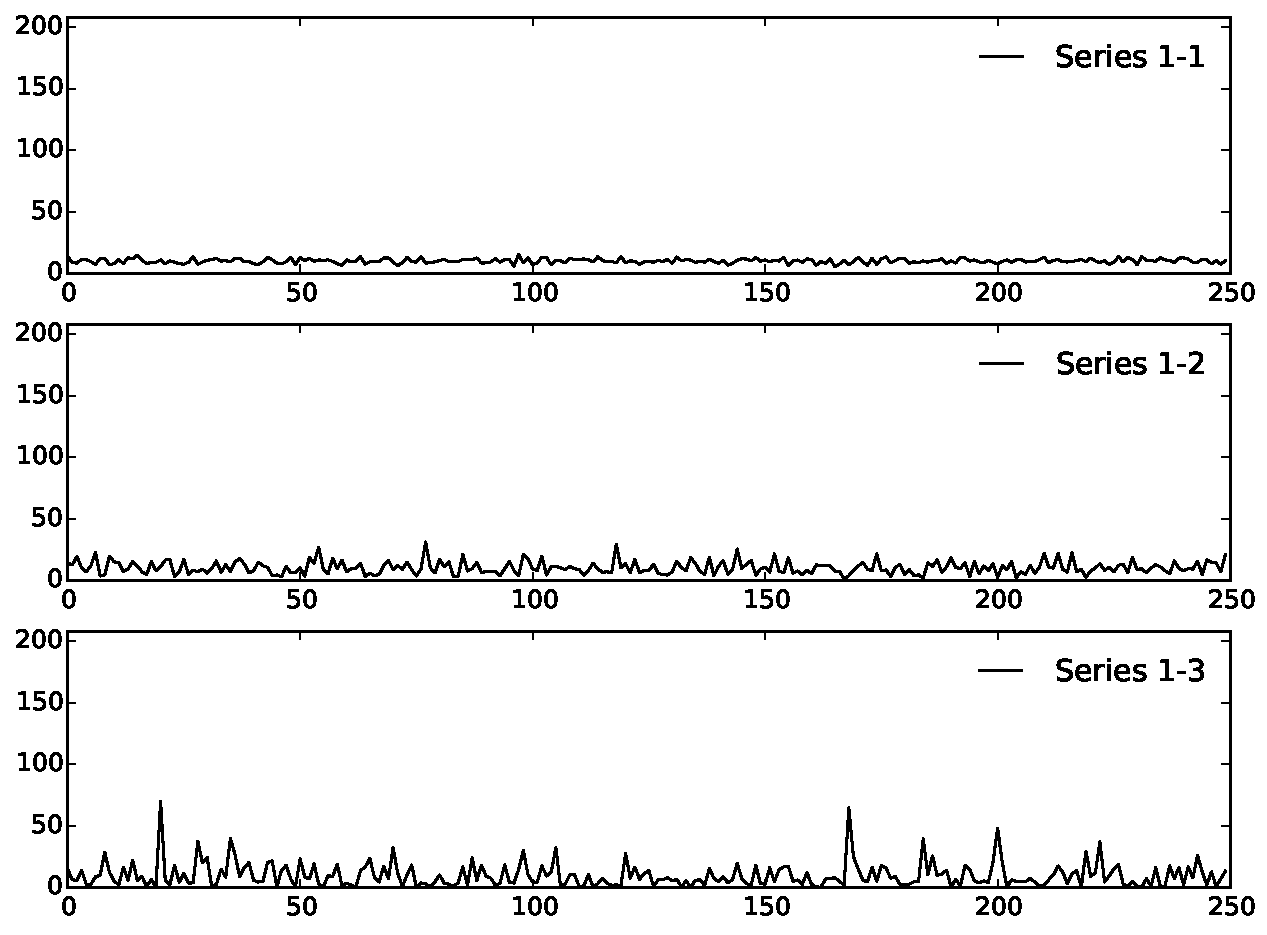
\includegraphics[width=.4\linewidth]{figures/Patterns_1.pdf}
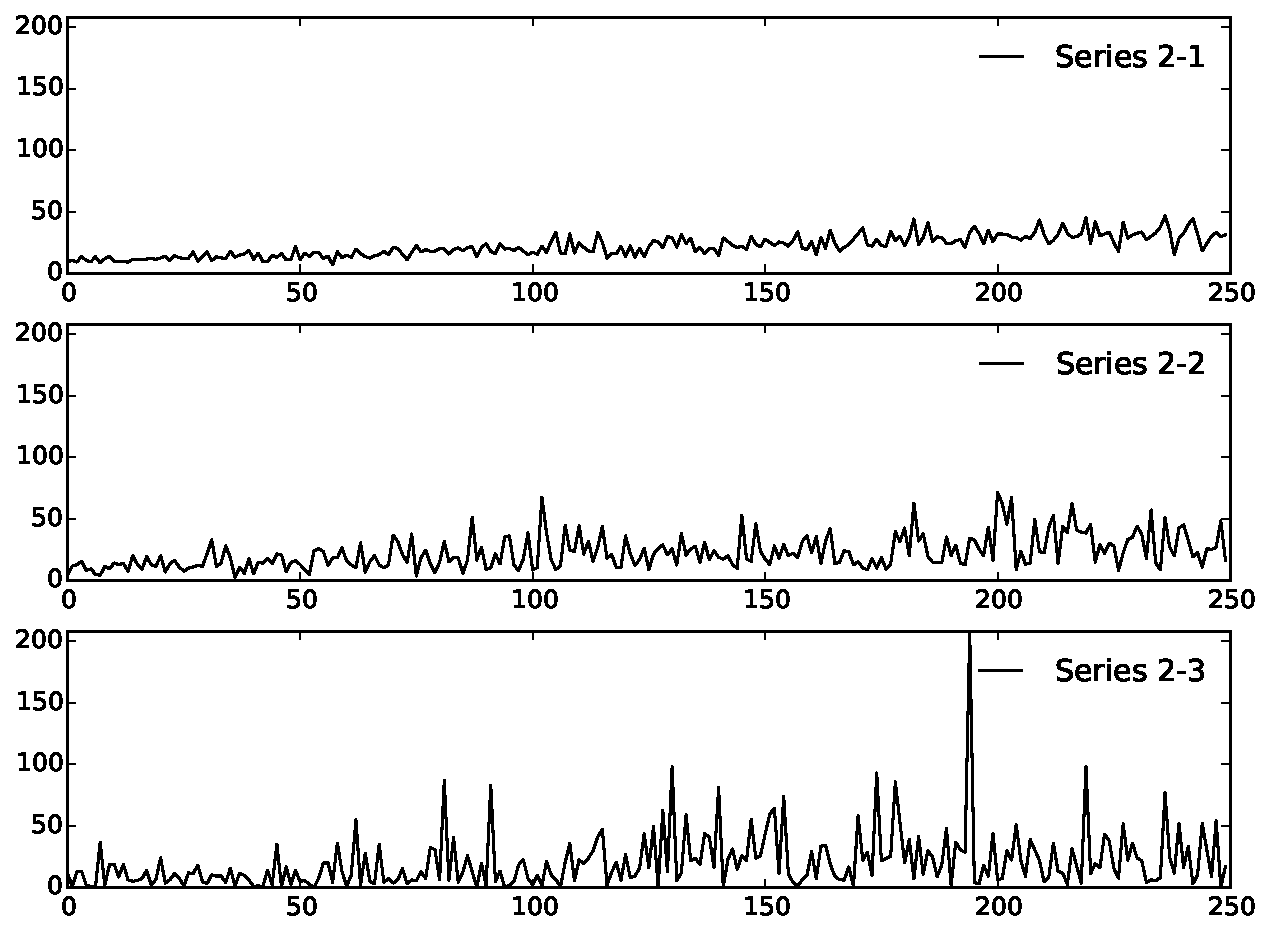
\includegraphics[width=.4\linewidth]{figures/Patterns_2.pdf} \\
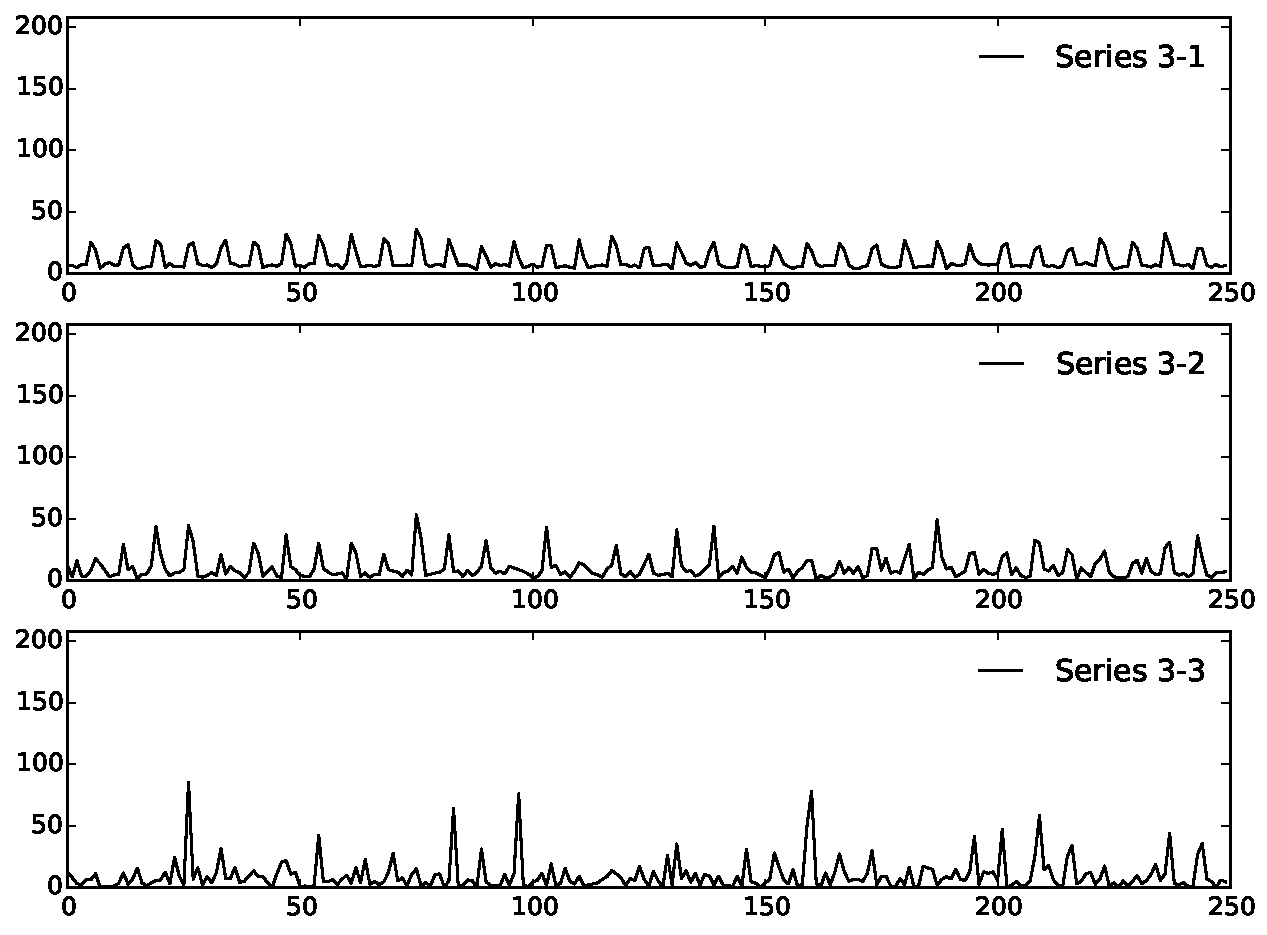
\includegraphics[width=.4\linewidth]{figures/Patterns_3.pdf}
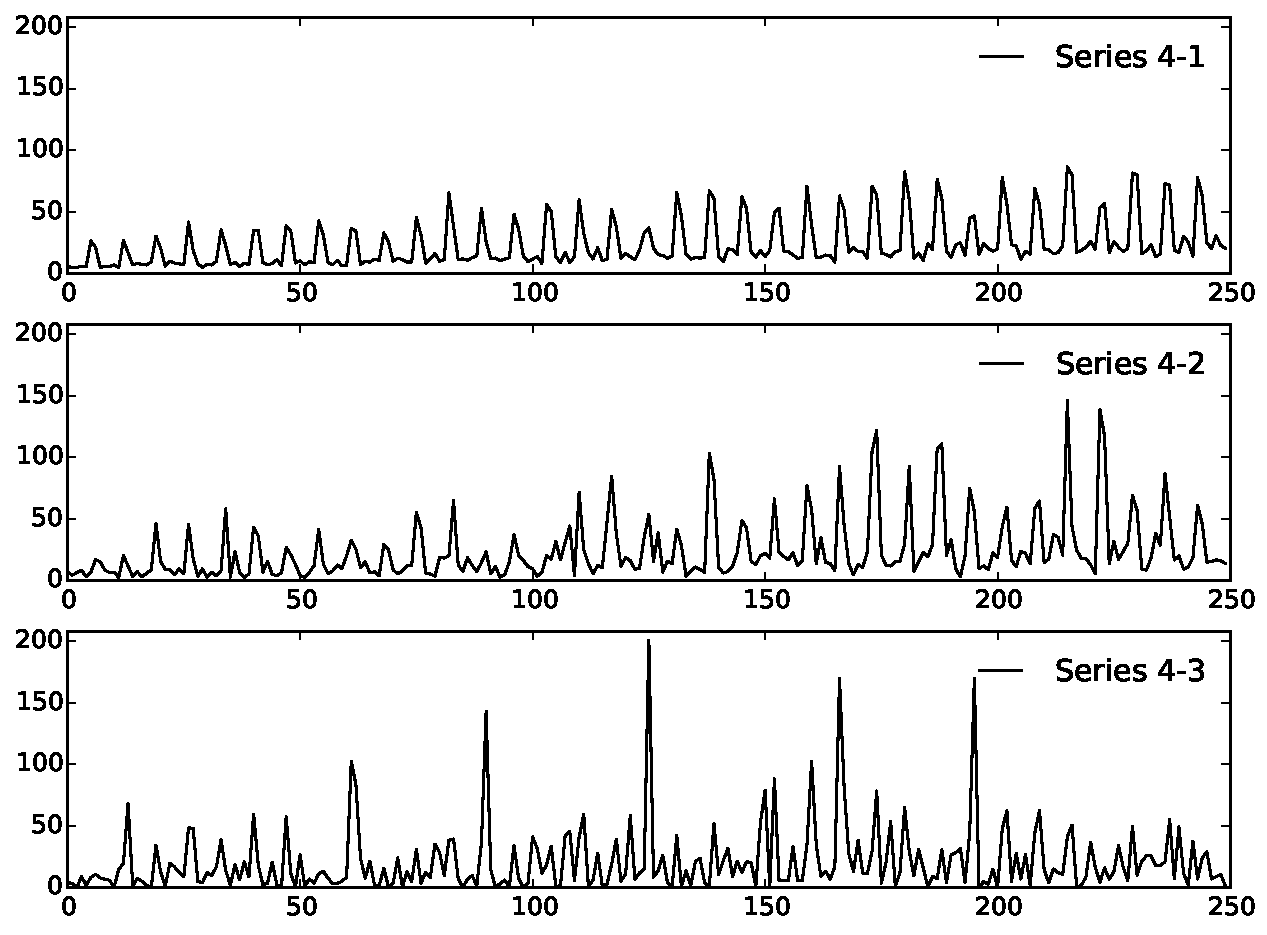
\includegraphics[width=.4\linewidth]{figures/Patterns_4.pdf}
\caption{Exercise~\ref{plots} plots}
\label{fig:plots}
\end{figure}
\end{landscape}
\newpage

%\begin{landscape}
%\let\thefootnote\relax\footnotetext{\textbf{Question~\ref{inter}}}
%
%\begin{center}
%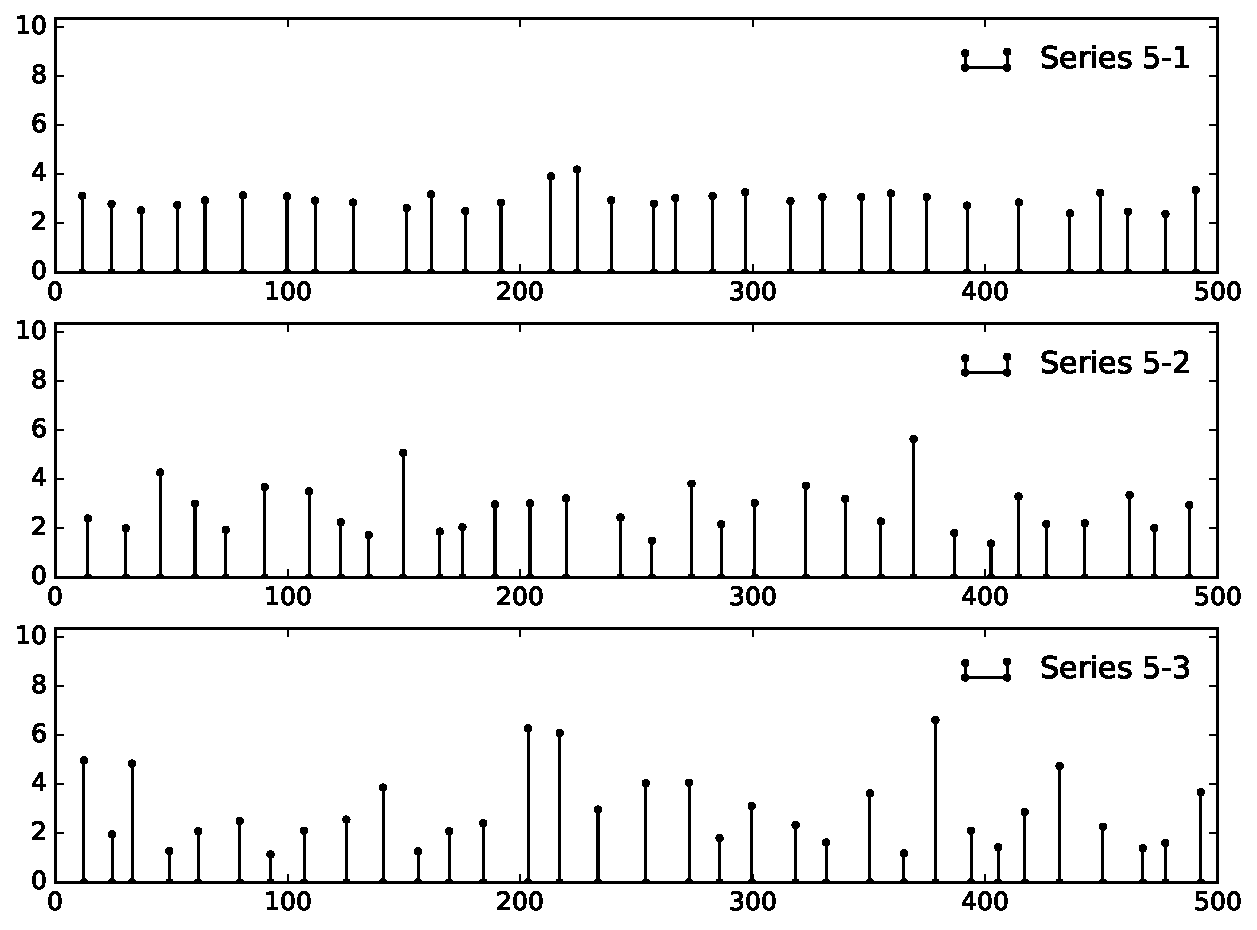
\includegraphics[width=.49\linewidth]{figures/Intermittent_1.pdf}
%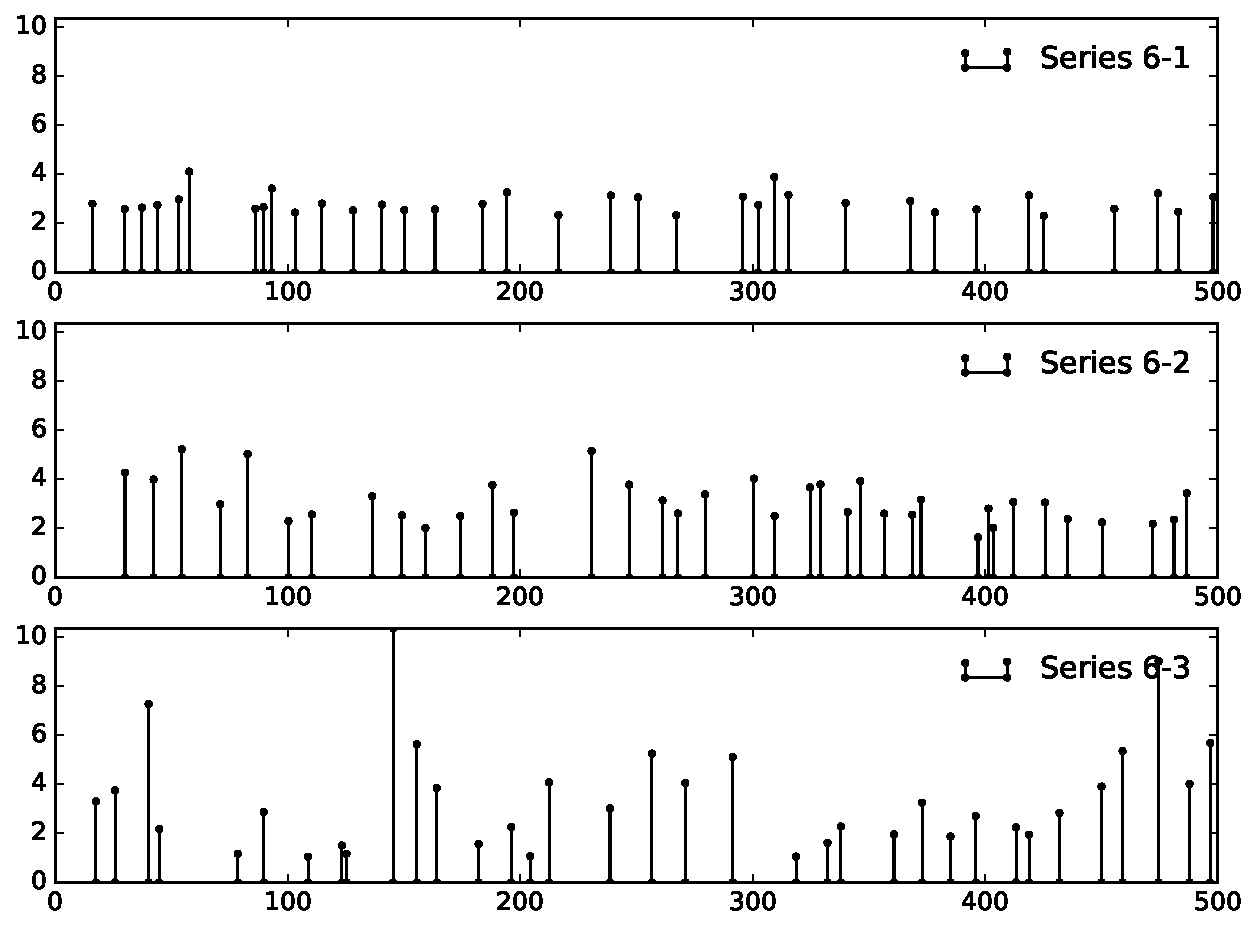
\includegraphics[width=.49\linewidth]{figures/Intermittent_2.pdf} \\
%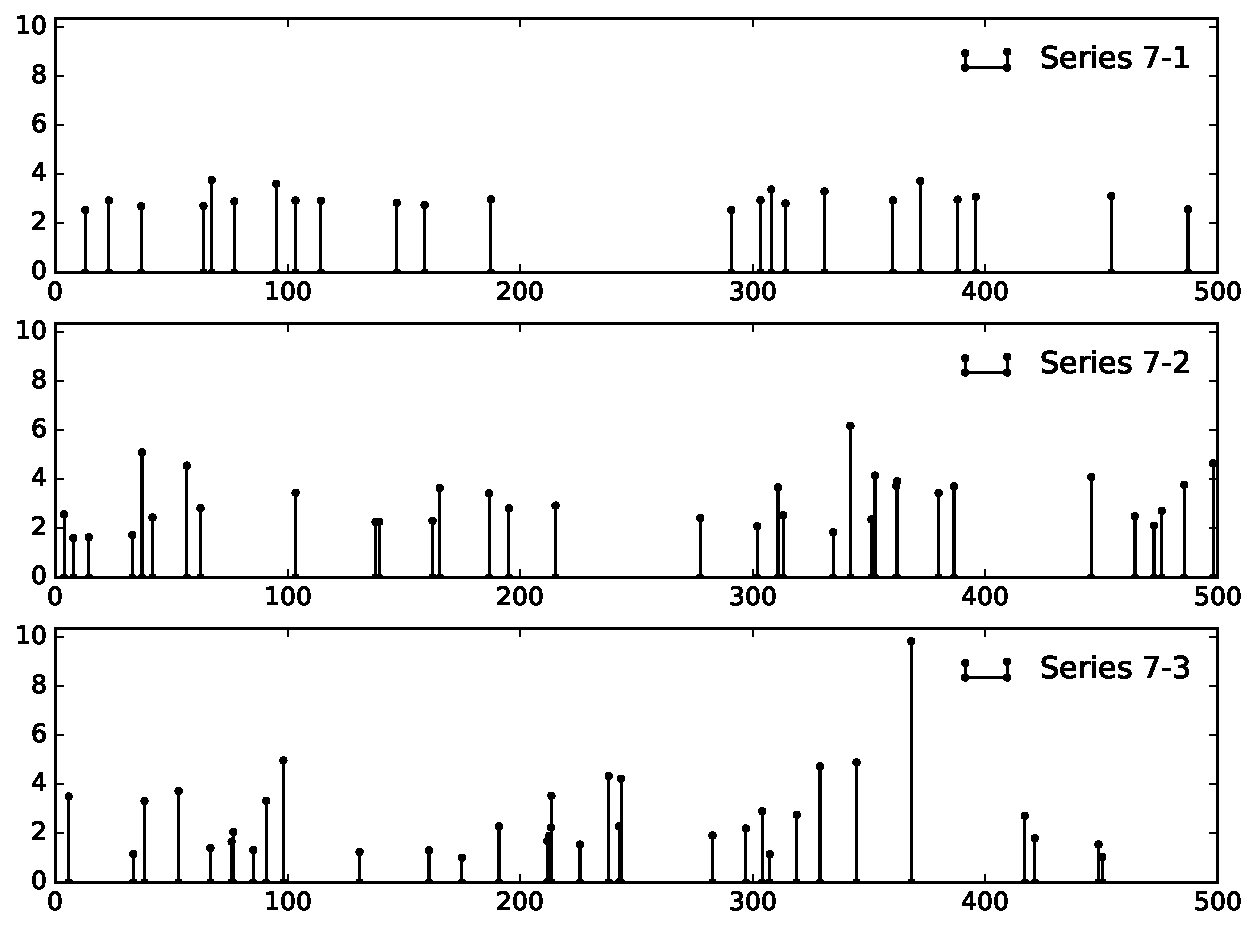
\includegraphics[width=.49\linewidth]{figures/Intermittent_3.pdf}
%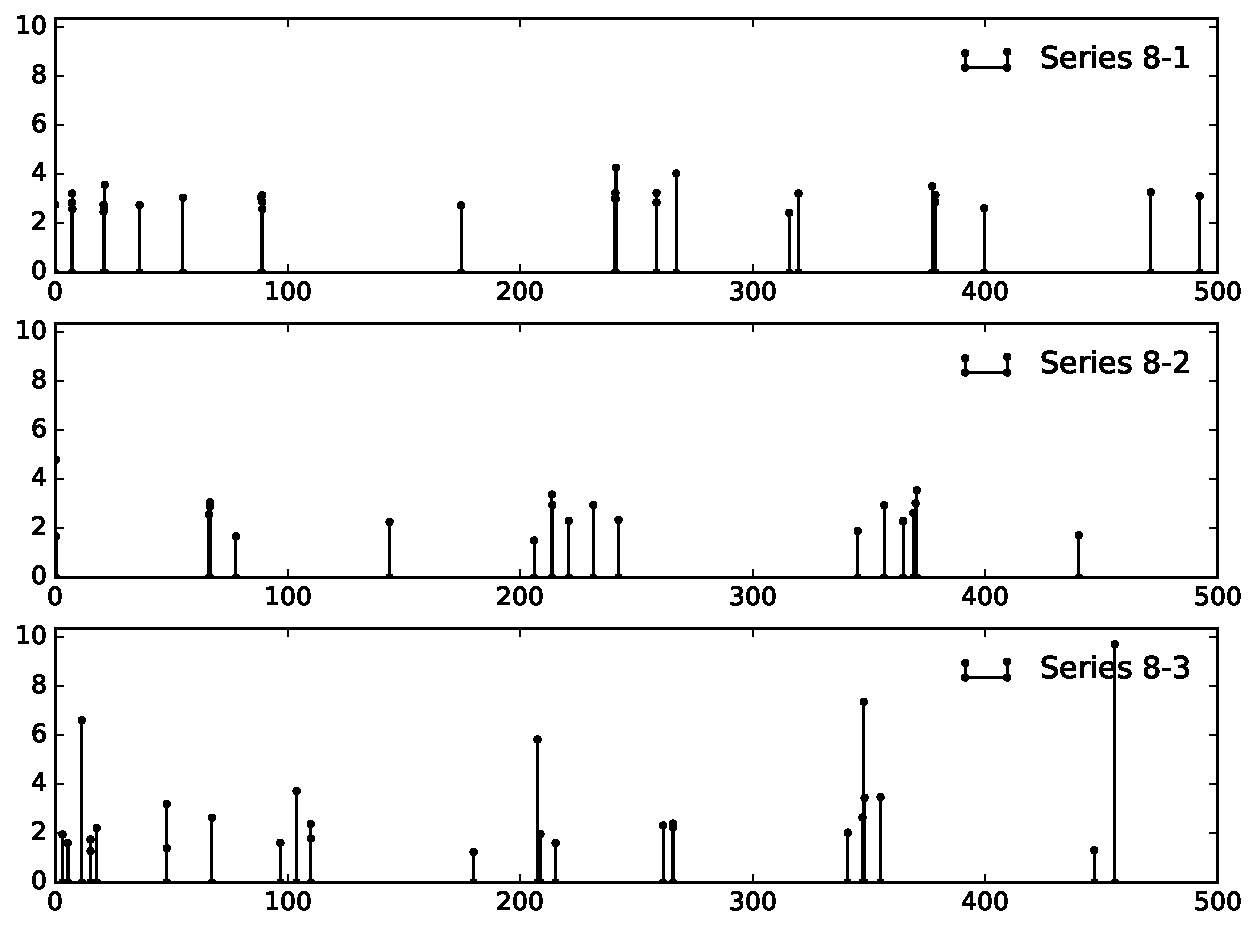
\includegraphics[width=.49\linewidth]{figures/Intermittent_4.pdf}
%\end{center}
%\end{landscape}





%\begin{exercise}
%The EOQ model is based on the assumption that the fixed ordering cost is independent of the order quantity. Consider the following variant of the model where this assumption is not valid anymore. Here, if the order quantity is less than or equal to $Q^{\max}$, then the fixed ordering cost will be $A_1$, and it will be $A_2$ otherwise. 
%
%\begin{enumerate}
%\item Develop a procedure to find the optimal order quantity for this variant of the EOQ model.
%\item Assume that the demand $D$ that is used in computing the order quantity is off by a factor of $\Delta$. That is, actual demand happens to be $D(1+\Delta)$ rather than $D$. 
%
%\end{enumerate}
%
%We have the following data: $A_1=50$, $A_2=85$, $Q^{\max}=100$, $h=2$, $D=1000$. 
%
%
%(for the sake of simplicity neglect the unit production cost)
%
%Now assume that the demand $D$ that is used in computing the order quantity is off by a factor of $\Delta$. That is, actual demand happens to be $D(1+\Delta)$ rather than $D$. 
%
%  \begin{solution}
%TBD
%
%\begin{center}
%\includegraphics[width=.5\linewidth]{figure_2.pdf}
%\end{center}
%  \end{solution}
%\end{exercise}
%




%
%
%Forecast approaches
%Extrapolation of historical data
%• Time series
%• Regression
%• Smoothing
%• Forecasts based on other factors
%• Promotions
%• Substitution effects
%• Dependent items (MRP)
%• Economic conditions
%• Expert knowledge
%
%
%Phases in identifying and using a forecasting model
%1. Pattern recognition (level, trend, season, shift)
%2. Factor initialization (level, trend factor, seasonal effect)
%3. Select time series forecasting model (e.g., mov. average, exp sm.)
%4. Develop forecasting model over time by updating factors (level,
%trend, season) after new data has become available
%5. Optimize forecasting parameters (n,α,β,γ) using criterion (e.g.,
%MSE or MAPE) based on subset of data
%6. Test forecasting model on complete dataset (i.e., are the errors
%independently normally distributed –you are ready-or did we miss a
%pattern –return to 1-?)





%Lead time
%› What lead time to use in our models?
% Lead time from supplier to inventory?
% Lead time from inventory to customer?
%› How to express lead times?
% Working days?
% Calendar days?
% Days, Weeks, Months, Years?
%
%How to model lead times?
% Constant or zero
% Dynamically varying (e.g. seasonal patterns)
% Stochastically varying (beware of crossovers)
%
%lead time in inventory models:
%the time between
%the moment a decision is made to issue an order
%and
%the first moment when a not-yet issued order is
%available for service to the customer
%
%
%Continuous and Periodic Review
%and Review period R: Risk period
%Length of time between successive observations
%of the inventory position (=“can order” moments)
%Continuous inventory control: R=0
%Periodic inventory control: R>0
%Is the review period included in the lead time?
%
%
%Review period and Risk period
%The current order should cover demand +
%uncertainty up till earliest arrival of next order:
%If R=0: Next order moment when demand occurs
%Risk period = L
%If R>0: Next order moment after R periods
%Risk period = L+R
%“Lead time demand”=demand during the Risk period
%
%Lead time demand distribution
%Risk period demand distribution
%› Text book approach:
%› Convolution of
% constant lead time (risk period) L
% stationary independent demand distribution
%- stationary means: no trends, no seasons
%- independent means: demand in one period
%does not depend on demand in other periods
%- constant mean μ, standard deviation σ / period
% Lead time demand ~(L*μ; σ√L)
%
%
%Lead time demand distribution
%Risk period demand distribution
%› Problems:
% Are risk periods constant?
% Is demand per period stationary?
% Is demand information per period independent?
%› Solutions:
% Model uncertainty in lead times/risk periods
% Use stationary forecast errors per period
% Forecast for whole lead time (risk period) ahead
%
%
%Lead time demand distribution
%Risk period demand distribution
%› Use of forecast and forecast error in
%non─stationary demand distribution
%› If forecasting has resulted in normal distributed
%forecast error:
% Use forecast next period as estimator of the
%expected demand in that period
% Use Root Mean Squared Error as initial estimator
%of the standard deviation of the expected demand
% Correct standard deviation based on lead time
%length and smoothing parameter used
%
%
%Lead time demand distribution
%Risk period demand distribution
%› Forecasting may NOT result in normal
%distributed forecast error if:
% Number of observations is too small (<30)
% Mean demand per period is too small (<10)
% Coefficient of variation (σ/μ) > 0.5
%› Other lead time demand distributions:
% Poisson (discrete distribution if demand < 10)
% Lognormal or Gamma (avoid negatives)
% Bootstrapping (sampling from original data)
%
%
%Service levels
%How to measure service of an inventory system?
%› Service to whom?
%› Service from where?
%› Service time limited?
%› Partial deliveries?
%› Differences in service over time?
%
%Two inventory control service levels measure
%differences in service over time.
%› P1: Service level per cycle
%› P2: Fill Rate
%
%P1: Service level per cycle
%Cycle starts when Q arrives
%Cycle ends when next Q arrives
%Frequency of stockout
%at the end of a cycle
%How many cycles for
%good measure?
%
%
%P2: Service level: Fill Rate
%% demand that can be fulfilled from stock
%30
%P1
%P2
%• Better relation with
%experienced service
%by customer
%• Easier to show trend
%in service over time
%• Lower safety stock
%required
%• Calculations more
%complex
%|
%
%Summary
%› Coping with intermittent demand
%› Focus on time horizon for which we need forecasts
% Lead time
% Review Period
%› What to do if forecast errors are not normal, but
%no further patterns to be included in model?
%› What service level is appropriate?





%\section{Week 3 of Jan's lecture}
%\label{sec:week-3-jans}
%
%
%
%Inventory points, Lead times, I/O interface
%• Inventory Control Models
%• Objective
%• Decision Variables
%• Constraints
%• Parameters
%• Assumptions
%• Periodic review or continuous review
%• Other models
%• Calculating P1 and P2 service level
%
%
%There are typically mutliple inventory points to consider
%\begin{itemize}
%\item From supplier to RMI
%\item From RMI to CODP
%\item From CODP to FGI
%\item From FGI to customer
%\end{itemize}
%make clear what lead time you consider
%
%How to control the lead time ..
% to the customer?
% from RMI to the CODP?
% from the supplier to the RMI?
%
%› If we would like to control inventory, we …
% choose a specific inventory point to control
% take decisions that affect the inventory at
%that point
% know how to measure the effectiveness of
%these decisions
%
%Inventory control
%What about the
%• Objective
%• Decision Variables
%• Constraints
%• Parameters
%• Assumptions
%
%
%
%Inventory Control
%What about uncertainty?
%• What parameters?
%• How to model?
%• Ignore
%• Include
%
%me
%› Continuous review (Q,r) model: order Q if IP≤r
% R
%R+Q
%L L
%Inventory position
%Inventory level
%Time
%SS
%0
%W
%
%\section{Week 4}
%\label{sec:week-4}
%
%ABC classification (Teunter et al., 2010)
%• Service level optimisation (Teunter et al., 2010)
%• Multi-item problems
%• Commonality (Baker et al., 1986)
%• Perishability
%
%ABC according to APICS
%ABC classifies a group of SKUs in
%decreasing order of annual dollar volume
%(price multiplied by projected volume) or
%other criteria. This array is then split into
%three classes, called A, B and C.
%(Blackstone and Cox, 2008)
%
%The standard practice is to assign the same
%service level to each SKU in a particular class
%Lee - NONSTOP solutions
%Pflitsch - SLIMSTOCK
%
%Which class should get the highest service level?
%› Some authors have argued that A items are
%the most critical for a firm.
%› Others have claimed that dealing with
%stockouts is not worth the effort for C items.
%Hopp \& Spearman:
%It makes sense to use sophisticated time-consuming techniques to
%tightly coordinate the arrival of A-parts, not for C-items.
%Slack et al.:
%Different inventory management decision rules are needed for
%different classes of inventory
%
%Service Level P2 – Fill Rate
%› The fill rate (FR) is the fraction / percentage of
%customers satisfied directly from stock on hand.
%› It is the most widely applied service level measure.
%› Although the calculations to find k are more
%complex, the good news is that software can do this!
%› But software does not tell you what an appropriate
%fill rate is and whether it should be the same for
%every SKU!
%
%Multiple items
%Service levels for demand for multiple items:
%Volume Fill rate = fraction of demanded units
%available from stock on hand
%Or
%Order line Fill rate = fraction of order lines
%that are completely available from stock on
%hand
%Or
%Order Fill rate = fraction of orders completely
%available from stock on hand




\subsection{From Forecasts to Demand Distributions}

\begin{exercise}
What is the added value of considering stochastic demands? What if we simply use our forecast for planning?


\begin{solution}
Let's begin with this: 'Forecasts are always wrong!' and 'Forecast errors are costly!'. Therefore, our models should acknowledge the fact that forecasts can be wrong. Furthermore, some forecast errors are more costly than others, e.g. over-forecast vs under-forecast. If the forecast is larger than the demand, then we have an overage cost (procurement in advance, holding, obsolescence); and if forecast is lower than the demand then we have a shortage cost (backorder cost, not meeting service quality target, loss of revenues). Often the shortage cost beat the overage cost. As a result of this, if real demand is distributed around some mean value, you order more than the mean. This is often referred to as the 'safety stock'. 

To sum up, we need to integrate not only the the forecast but also the extent and the direction of the forecast error into our planning, as doing otherwise might have financial consequences. 
\end{solution}
\end{exercise}

\begin{exercise}
I am confused. I thought that we were forecasting to predict the demand. What forecast errors have to do with that?


\begin{solution}
To answer this, we need to better understand what a forecast stands for. There is no perfect forecast as demand is inherently uncertain. Therefore, it is 'very normal' to have forecast errors. The question is whether your forecast errors match the inherent uncertainty in demand. That is, whether your forecast errors  originate from the demand uncertainty or they are the result of using a bad forecasting method. If it is the former, then you can safely assume that your point forecast is the average demand and your forecast errors are variations of demand from its average. If it is the latter, then you should do your best to devise a better forecasting method.

Let us illustrate this with a simple example. Assume that demand is either 0 or 1, and the inherent uncertainty of the demand comes from a coin toss. That is, demand is 1 if it is heads and it is 0 if it is tails. As a planner; you do not know that demand indeed follows a coin toss, yet you need to forecast the demand. It is easy to see that there is no forecasting method you can use to predict the demand with certainty. In fact, the 'best' you can expect from a forecasting method is to tell you that the probability of having a demand of 0 units and 1 units are both 50\%. Here, if your forecast model provides a forecast error of 0.5 (almost) half of the time and -0.5 in the other half, then you are already there. Despite the sizeable amount of forecast errors, your forecasting method is just fine. On the other hand, if your forecast errors are, for instance, increasing or decreasing over time or have a tendency to be higher every two periods, then there is something wrong with your forecast method that should be repaired.

Back to the original question; forecasts help us to predict average demand and it's variability from this average. Therefore they provide us the grounds for managing inventories. 
\end{solution}
\end{exercise}

\begin{exercise}
How can we measure or assess the demand uncertainty?


\begin{solution}
The answer can be found in the 'probability theory'. We can capture the uncertainty in demand through its probability distribution.
\end{solution}
\end{exercise}

\begin{exercise}
What is a demand distribution?


\begin{solution}
We should start with defining demand (over a pre-specified interval of time) as a random variable. Let this variable be $D$. Then, the (cumulative) distribution function of $D$ is given by $F(x)=\P{D\leq x}$. That is, the probability that demand being less than or equal to some constant $x$. 
\end{solution}
\end{exercise}

\begin{exercise}
How can we derive a demand distribution using forecasts? 


\begin{solution}
There is no theoretically supported procedure for this purpose. A common approach is to approximate the variation of the demand with the variation of the forecast. To that end, first you need to make sure that the forecast indeed captures the trend and/or seasonality in the demand. This is the case if your forecast errors are relatively unbiased and do not follow a pattern over time. Then, you can approximate the mean demand with your point forecast and its deviation with the forecast errors. For instance; if your forecast errors are normally distributed over time, then you can assume that demand is normally distributed. Normal distribution is characterized by two parameters: mean and standard deviation. Then you can set the mean as your forecast and let the standard deviation be the square root of the mean squared error of your forecast. If your forecast errors are not normally distributed, then you can try and fit them to another distribution and/or use the empirical distribution (i.e. the distribution that you have observed). 

Note that forecasting itself can be quite involved in many cases; for instance, where demand is auto-correlated and/or influenced by parameters that are not a part of your data. In such cases, standard time-series forecasting methods may not provide good forecasts at all. However, these issues are beyond the scope of this course. 
\end{solution}
\end{exercise}

\begin{exercise}
What is the difference between the demand distribution and the lead time demand distribution?


\begin{solution}
We construct demand distributions for demand over a given interval of time. If that interval is the lead time, then we simply have the lead time demand distribution. There are two possible ways of approaching the lead time demand distribution. First, you can start with forecasting the demand over a period and derive its distribution as usual and then use this distribution to construct the lead time demand distribution. For instance, if demand over a period is normally distributed with mean $\mu$ and standard deviation $\sigma$, then demand over $n$ periods (assuming that the demand in these periods follow the same distribution) is also normally distributed with mean $n\cdot\mu$ and standard deviation $\sqrt{n}\cdot \sigma$ (this property holds only for normal distribution). Second, you can directly start by forecasting the lead time demand rather than the period demand and derive its distribution.
\end{solution}
\end{exercise}

\begin{exercise}
It appears that normal distribution comes in handy. How can you check whether a data set is normally distributed?


\begin{solution}
There are many ways. There are very practical visual approaches, such as plotting the data as a histogram and checking against the normal distribution curve and making use of a normal distribution QQ-plot. Also, there are well-known statistical tests such as Shapiro-Wilk, Kolmogorov-Smirnov, and Anderson-Darling.
\end{solution}
\end{exercise}

\begin{exercise}
Are there other distributions that are commonly used in inventory control, besides normal distribution?


\begin{solution}
Normal distribution often does not work with slow movers, i.e. products with infrequent demands. For instance, if a product is sold only a few times over the lead time, it would not make sense to assume demand is normally distributed. In such cases Poisson distribution can be an option. 

The preference towards normal and Poisson distributions is not only due to their 'nice' mathematical characteristics but also their power in capturing real-life demand data.
\end{solution}
\end{exercise}


\Closesolutionfile{ans}
\opt{solutionfiles}{
\subsection{Solutions}
\input{ans}
}

\clearpage

%%% Local Variables:
%%% mode: latex
%%% TeX-master: "inventory_notes"
%%% End:
